%% PREAMBLE
\documentclass[xcolor=dvipsnames,10pt]{beamer}
\setbeamercovered{transparent} % dim inactive elements

% general theme
\usetheme{Madrid}

% inner theme
\useinnertheme{circles}

% color scheme
\definecolor{UBCblue}{rgb}{0.04706, 0.13725, 0.26667}
\definecolor{UBCgrey}{rgb}{0.3686, 0.5255, 0.6235}
\setbeamercolor{palette primary}{bg=UBCblue,fg=white}
\setbeamercolor{palette secondary}{bg=UBCblue,fg=white}
\setbeamercolor{palette tertiary}{bg=UBCblue,fg=white}
\setbeamercolor{palette quaternary}{bg=UBCblue,fg=white}
\setbeamercolor{structure}{fg=UBCblue}
\setbeamercolor{section in toc}{fg=UBCblue}
\setbeamercolor{subsection in head/foot}{bg=UBCgrey,fg=white}

% turn off ugly footer
\setbeamertemplate{footline}[frame number]{}
\setbeamertemplate{navigation symbols}{}

% fonts
\usefonttheme{professionalfonts} % using non standard fonts for beamer
\usefonttheme{serif} % default family is serif
\usepackage{fontspec}
\setmainfont{Liberation Serif}

% hyphenation for letterspacing and text decoration
\usepackage{soul}

% references
\usepackage[backend=biber,style=authoryear-icomp]{biblatex}
\addbibresource{bibl.bib}
\makeatletter
\renewrobustcmd{\blx@mkbibfootnote}[2]{%  deal with columns
  \iftoggle{blx@footnote}
    {\blx@warning{Nested notes}%
     \addspace\mkbibparens{#2}}
    {\unspace
     \ifnum\blx@notetype=\tw@
       \expandafter\@firstoftwo
     \else
       \expandafter\@secondoftwo
     \fi
       {\csuse{blx@theendnote#1}{\protecting{\blxmkbibnote{end}{#2}}}}
       {\csuse{footnote#1}[frame]{\protecting{\blxmkbibnote{foot}{#2}}}}}}
\makeatother

% SI units in text and stuff related to math, tables, etc.
\usepackage[detect-all]{siunitx}
\sisetup{per-mode=symbol,range-phrase=--,range-units=single,list-units=single}
\usepackage{amsmath, amsfonts, amssymb}
\usepackage{bm}
\usepackage{nicefrac}
\usepackage{multirow}

% figures
\usepackage{tikz}
\usetikzlibrary{calc, positioning, shapes, backgrounds, fit, arrows}
\usepackage{pgf-spectra}
\usepackage{contour}
\usepackage{adjustbox}
\usepackage{wrapfig}
\def\checkmark{\tikz\fill[scale=0.4](0,.35) -- (.25,0) -- (1,.7) -- (.25,.15) -- cycle;}
\usepackage{caption}
\captionsetup[figure]{labelformat=empty} %  removes "figure" tag from the caption
\captionsetup{justification=centering} % caption centering
\usepackage[labelformat=empty]{subcaption}

% title
\setbeamertemplate{title page}[default][wd=\textwidth,rounded=false]
\title{Advanced Technique for Assessment of Spatially Averaged Dosimetric Quantities on Nonplanar Surfaces}
\author[Ante Kapetanović]{Ante Kapetanović}
\institute{Faculty of Electrical Engineering, Mechanical Engineering and Naval Architecture (FESB)}
\date{September 25, 2023}
\titlegraphic{\includegraphics[height=1.25cm]{artwork/logo/unist.png}}


%% DOCUMENT
\begin{document}


% generate the title slide
\begin{frame}[plain]
    \maketitle
    \begin{center}
        \scriptsize{%
            Jury Members\par
            President: Prof. Zoran Blažević, PhD\par\medskip
            \begin{table}
                \centering
                \begin{tabular}{llll}
                Examiners: & Prof. Zvonimir Šipuš, PhD & Supervisor: & Prof. Dragan Poljak, PhD \\
                 & Assoc. Prof. Kun Li, PhD &  &  \\
                 & Assoc. Prof. Vicko Dorić, PhD &  &  \\
                 & Assoc. Prof. Mario Cvetković, PhD &  & 
                \end{tabular}
            \end{table}
        }%
    \end{center}
\end{frame}

% the main table of contents
\begin{frame}{Table of contents}    
    \setbeamertemplate{section in toc}[sections numbered]
        \tableofcontents
\end{frame}

% a table of contents that appear before new section
\AtBeginSection[]{
    \begin{frame}{Table of contents}
        \setbeamertemplate{section in toc}[sections numbered]
        \tableofcontents[currentsection,hideallsubsections]
    \end{frame}
}



% introductory section
\section[Introduction]{Introduction}

\subsection{Problem and subject of scientific research}
\begin{frame}{Problem and subject of scientific research}
    \begin{itemize}
        \item The rise in the number of data-intensive wireless devices $\rightarrow$ expansion of the utilized radio frequency (RF) spectrum into millimeter waves (MMW)\footcite{Rappaport2013Millimeter}
        \item Global roll-out of the fifth-generation (5G) standard for broadband cellular networks $\rightarrow$ improved communication performance by increasing channel capacity and reducing network latency through\footcite{Andrews2014What}
        \begin{itemize}
            \item carrier aggregation,
            \item multiple-input multiple-output (MIMO) technology,
            \item beam-forming, i.e., the spatial filtering,
            \item utilization of frequency range (FR) 1 (\SIrange{0.45}{6}{\GHz}), FR 2 (\SIrange{24.25}{52.6}{\GHz})
        \end{itemize}
        \item Increased public interest in (and concerns about) the potential adverse health effects from exposure to RF electromagnetic (EM) radiation\footcite{Wu2015Safe}
    \end{itemize}
\end{frame}

\begin{frame}{But what is EM radiation?}
    \input{artwork/em_spectrum.tex}
\end{frame}

\begin{frame}{Non-ionizing EM radiation effects
on biological tissue}
    \begin{itemize}
        \item \emph{Biological effect} $\rightarrow$ any induced (physical, chemical, or mechanical) change in tissue\footcite{ICNIRP2020Principles}
        \item Feedback repair mechanism $\rightarrow$ preservation of homeostasis within \emph{threshold limits}
        \item Limits exceeded $\rightarrow$ \emph{adverse health effect}\footcite{WHO2022Health}
        \item Interaction effects are frequency-dependent
        \begin{tabular}{p{2.7cm}p{8cm}}
            static fields & induced fields and currents within tissue\\
            \SIrange{0}{0.1}{\MHz} & stimulation of excitable cells\\
            \SIrange{0.1}{10}{\MHz} & stimulation of excitable cells, tissue heating\\
            above \SI{10}{\MHz} & tissue heating exclusively
        \end{tabular}
        \item Increase in frequency $\rightarrow$ absorbed power is dissipated predominately across the surface of the exposed tissue\footcite{Ziskin2018Tissue}
        \end{itemize}
\end{frame}

\begin{frame}{Exposure limits to artificial EM fields}
    \begin{itemize}
        \item Prescribed by international guidelines\footcite{ICNIRP2020Guidelines} and standards\footcite{IEEE2019Standard}
        \item Offer a protection against the possibility of occurrence of adverse health effects by
        \begin{itemize}
            \item identifying established mechanism of biological interaction,
            \item setting allowable limits of exposure,
            \item applying safety factors in a conservative manner to account uncertainty
        \end{itemize}
        \item Derived threshold values $\rightarrow$ \emph{basic restrictions} or (BR) $\rightarrow$ \emph{reference levels} (RL)
        \begin{itemize}
            \item whole-body or local exposure
            \item brief or steady-state exposure
        \end{itemize}
        \item \emph{Specific absorption rate} (SAR) was used as the BR for the steady-state core (whole-body average) and local (10-g or 1-g average) temperature rise from \SI{100}{\kHz} to \SI{300}{\GHz}
    \end{itemize}
\end{frame}

\begin{frame}{Exposure assessment and dosimetry in the era of 5G}
    \begin{columns}[c]
        \begin{column}{0.5\textwidth}
             \begin{itemize}
                \item<1> At \SI{6}{\GHz}, \SI{90}{\percent} of the power is absorbed within the uppermost layer of the exposed tissue
                \item<2> BR are set in terms of the area-averaged \emph{absorbed power density} (APD)
                \item<3> Line integral of SAR depth-wise into the tissue $\rightarrow$ \emph{transmitted power density} (TPD)
                \item<4> Area-averaged TPD $\equiv$ area-averaged APD $\rightarrow$ consistency and continuity with volume-averaged SAR
            \end{itemize}
        \end{column} 
        \begin{column}{0.5\textwidth}
            \begin{onlyenv}<1>
                \begin{center}
                \begin{figure}
                    \includegraphics[width=\textwidth]{artwork/penetration_depth.pdf}
                    \caption{Penetration depth and transmission coefficient as a function of frequency}
                \end{figure}
                \end{center}
            \end{onlyenv}
            \begin{onlyenv}<2>
                \begin{center}
                \begin{figure}
                    \includegraphics[width=0.85\textwidth]{artwork/averaging_surface.a.pdf}
                    \caption{Evaluation surface on a multiple-layer tissue-equivalent block model}
                \end{figure}
                \end{center}
            \end{onlyenv}
            \begin{onlyenv}<3>
                \begin{center}
                \begin{figure}
                    \includegraphics[width=0.7\textwidth]{artwork/averaging_surface.b.pdf}
                    \caption{Orthographic projection of the evaluation surface on a multiple-layer tissue-equivalent block model}
                \end{figure}
                \end{center}
            \end{onlyenv}
            \begin{onlyenv}<4>
                \begin{center}
                \begin{figure}
                    \includegraphics[width=0.75\textwidth]{artwork/averaging_volume.pdf}
                    \caption{A 10-g cubic volume for assessment of SAR during local steady-state exposure below \SI{6}{GHz}}
                \end{figure}
                \end{center}
            \end{onlyenv}
        \end{column}
    \end{columns} 
\end{frame}

\begin{frame}{Governing equations at gigahertz range -- APD}
    \begin{columns}[c]
        \begin{column}{0.4\textwidth}
            \begin{itemize}
                \item Recent versions of IEEE/ICES-2019 standard and ICNIRP-2020 guidelines propose two distinct definitions of APD
                \begin{enumerate}
                    \item<1> spatially averaged normal component of the time-averaged Poynting vector,
                    \item<2> volume-averaged power loss
                \end{enumerate}
            \end{itemize}
        \end{column} 
        \begin{column}{0.6\textwidth}
            \begin{onlyenv}<1>
                \begin{equation*}
                    \centering
                        S_\text{ab, s} = \frac{1}{2A} \iint_{A} \Re \left[ \mathbf{E} \times \mathbf{H}^* \right] \cdot \mathbf{n} \; \mathrm{d}A
                \end{equation*}
                \begin{itemize}
                    \item $\mathbf{E}$, $\mathbf{H}$ -- peak values of the complex phasor electric and magnetic field on the surface
                    \item $A$ -- frequency-dependent averaging area
                    \item $\mathbf{n}$ -- surface normal on $A$
                    \item $\mathrm{d}A$ -- integral area element
                \end{itemize}
            \end{onlyenv}
            \begin{onlyenv}<2>
                \begin{equation*}
                    \centering
                    S_\text{ab, v} = \frac{1}{A} \iint_{A} \int_{z} \rho \; \text{SAR} \; \mathrm{d}z \; \mathrm{d}A
                \end{equation*}

                \begin{equation*}
                    \centering
                    \text{SAR} = \frac{\sigma \left| \mathbf{E} \right|^2}{2\rho}
                \end{equation*}
                \begin{itemize}
                    \item $\mathbf{E}$ -- the peak value of the complex phasor electric field within tissue
                    \item $\sigma$ -- conductivity of tissue
                    \item $\rho$ -- tissue density 
                \end{itemize}
            \end{onlyenv}
        \end{column}
    \end{columns}
\end{frame}

\begin{frame}{Governing equation at gigahertz range -- IPD}
    \begin{itemize}
        \item IPD is the modulus of the time-averaged free-space Poynting vector
        \begin{equation*}
            \centering
            S_\text{inc} = \left| \mathbf{E} \times \mathbf{H}^* \right|
        \end{equation*}
        \item Various definitions of the spatially averaged IPD have been proposed and discussed\footcite{IEEE2021Guide} with the following two standing out in particular
        \begin{enumerate}
            \item spatially averaged normal component of the time-averaged Poynting vector
            \begin{equation*}
                \centering
                S_\text{inc, n} = \frac{1}{2A} \iint_{A} \Re \left[ \mathbf{E} \times \mathbf{H}^* \right| \cdot \mathbf{n} \; \mathrm{d}A
            \end{equation*}
            \item spatially averaged magnitude of the time-averaged Poynting vector
            \begin{equation*}
                \centering
                S_\text{inc, tot} = \frac{1}{2A} \iint_{A} \left| \mathbf{E} \times \mathbf{H}^* \right| \; \mathrm{d}A
            \end{equation*}
        \end{enumerate}
        \item Both defintions correlate well with temperature rise ($r > 0.75$)
    \end{itemize}
\end{frame}

\begin{frame}{Sizing the averaging area}
    \begin{itemize}
        \item \SIrange{2}{6}{\GHz} $\rightarrow$ peak value of the power density
        \item $\geq$ \SI{6}{\GHz} $\rightarrow$ averaging on \SI{4}{\cm\squared} square evaluation plane\footcite{Hashimoto2017averaging,Funahashi2018Averaging}
        \item $\geq$ \SI{30}{\GHz} $\rightarrow$ averaging on \SI{1}{\cm\squared} square evaluation plane in addition to account for narrow beam formation\footcite{Foster2016Thermal}
        \item Power density spatially averaged on \SI{1}{\cm\squared} area should not exceed twice the value of the \SI{4}{\cm\squared} area \footcite{ICNIRP2020Guidelines}
    \end{itemize}
\end{frame}

\subsection[Overview of the existing research]{Overview of the existing research}
\begin{frame}{Tissue models and evaluation surfaces}
    \begin{columns}[c]
        \begin{column}{0.5\textwidth}
            \begin{itemize}
                \item Above \SI{6}{\GHz}, flat tissue-equivalent single- or three/four-layer models commonly utilized\footcite{Zhadobov2011Millimeter}
                    \begin{itemize}
                        \item \textit{stratum corneum},
                        \item viable epidermis and dermis,
                        \item hypodermis,
                        \item muscle
                    \end{itemize}
                \item Dielectric properties $\leftarrow$ four-term Cole-Cole model\footcite{Gabriel1996Compilation}
                \item Averaging area construction on a planar evaluation surface $\rightarrow$ IEC/IEEE 63195-2:2022 standard
            \end{itemize}
        \end{column}
        \begin{column}{0.5\textwidth}
            \begin{center}
            \begin{figure}
                \includegraphics[width=0.75\textwidth]{artwork/Li2021Figure2_adjusted.pdf}
                \caption{Skin models with different tissue compositions and the exposure condition. Taken from the recent international inter-comparison study by Li et al. 2021.}
            \end{figure}
            \end{center}
        \end{column}
    \end{columns}
\end{frame}

\begin{frame}{Current state of the research: A short synthesis}
    \begin{itemize}
        \item Definition of the appropriate exposure metric at the \SIrange[]{1}{10}{\GHz} range\footcite{Anderson2010SAR,McIntosh2010SAR}
        \item Harmonization of the transition frequency for BRs between existing exposure limits\footcite{Colombi2015Implications,Thors2016Exposure,Xu2017Understanding}
        \item 10- and 1-g averaging volume $\rightarrow$ \SIlist{4;1}{\cm\squared} evaluation plane\footcite{Hashimoto2017averaging,Funahashi2018Averaging,Foster2016Thermal,Foster2017Thermal}
        \item First mention of the spatially averaged TPD on the skin surface as a metric to estimate surface temperature rise \SI{6}{\GHz}\footcite{Funahashi2018Area-averaged}
        \item Validity of the spatially averaged IPD\footcite{Sasaki2017Monte,Li2019Relationship,He2018RF,Diao2021Effect,Carrasco2019Exposure,Miura2021Power,Nakae2020Skin,Morimoto2022Assessment,DeSantis2022On} as RL by various experimental/numerical techniques
        \item Validity of the spatially averaged APD\footcite{Li2021Quantitative,Taguchi2022Computation,Li2023Calculated} as BR by using the heating factor\footcite{Foster2018Modeling}
    \end{itemize}
\end{frame}

\begin{frame}{Current state of the research: Beyond the state of the art}
    \begin{columns}[c]
        \begin{column}{0.5\textwidth}
            \begin{itemize}
                \item Nonplanar body parts (fingers\footcite{Li2012Mechanisms} or ears\footcite{Sacco2022Exposure}) with the curvature radius $\sim$ wavelength of the incident EM field $\rightarrow$ underestimation of the spatially averaged quantities
                \item Appropriate curved models currently discussed within a working group under IEEE-ICES TC95 SC6
                \begin{itemize}
                    \item canonical shapes, e.g., sphere\footcite{Kushiyama2022Absorbed,Kapetanovic2022Assessment} or cylinder\footcite{Diao2020Assessment,Kapetanovic2023Machine}
                    \item anatomical tissue models\footcite{Kapetanovic2023Area-averaged}
                \end{itemize}
            \end{itemize}
        \end{column}
        \begin{column}{0.5\textwidth}
            \begin{center}
            \begin{figure}
                \includegraphics[width=0.95\textwidth]{artwork/Diao2020Figure2_adjusted.pdf}
                \caption{Reference averaging volumes for different APD computation schemes in Diao, Rashed and Hirata 2020.}
            \end{figure}
            \end{center}
        \end{column}
    \end{columns}
\end{frame}

\subsection{Motivation, purpose and objectives of the research}
\begin{frame}{Motivation, purpose and objectives of the research}
    \begin{itemize}
        \item To conduct a \emph{comprehensive investigation into the influence of geometric features and surface morphology of tissue} on the value of APD and IPD above \SI{6}{\GHz}
        \item To develop an \emph{accurate numerical solver} for surface integrals of the power flow, regardless of underlying numerical/analytical techniques employed in EM simulations
        \item To develop a \emph{computationally efficient automated detection of the worst-case exposure scenario}---the ``hot-spot'' region---on the exposed tissue surface
    \end{itemize}
\end{frame}

\subsection{Hypotheses}
\begin{frame}{Hypotheses}
    \begin{enumerate}
        \item<only@1> Traditional flat surfaces for the spatial averaging of power densities are inadequate for RF EM fields with wavelengths comparable to the approximate curvature radius of a nonplanar body part being exposed
        \item<only@2> Anatomical models with irregularities and asymmetries characterized by intricate convex-concave tissue structures on the surface require high-fidelity numerical estimation of surface normal vectors
        \item<only@3> Heterogeneous EM absorption in the near field require evaluating the spatially averaged power density over the entire outer surface of a nonplanar body part being exposed
    \end{enumerate}
    \begin{block}{Assumption 1}<1->
        Cylindrical or spherical models are superior for practical compliance assessment of exposure of common nonplanar body parts, e.g., fingers, outer ear, head, \dots
    \end{block}
    \begin{block}{Assumption 2}<2->
        Distribution of surface normal vectors affects the absorption of incident EM fields significantly 
    \end{block}
    \begin{block}{Assumption 3}<3->
        Hybridization of machine learning and traditional numerical methods enhances dosimetry analysis and enables the identification of worst-case exposure scenario without any priors
    \end{block}
\end{frame}

% materials and methods section
\section[Materials and methods]{Materials and methods}

\begin{frame}{Overview of the methodology}
    \begin{itemize}
        \item Development of the appropriate averaging method on curved, canonical surface (IEEE-ICES TC95 SC6 working group on power-density averaging)
        \item Spatial averaging on anatomical models -- highly dependent on the underlying numerical method and the software used during EM simulations
        \item Estimation of surface normals -- crucial for accurate assessment of the surface integrals representing the spatially averaged IPD/APD
        \item Effective construction of the averaging area and the spatial averaging of the surface-normal propagation-direction power density into the evaluation surface
        \item Fast and plausible algorithm to extract the ``hot-spot'' region which yields the peak spatial-average power density
    \end{itemize}
\end{frame}

\subsection{Nonplanar models}
\begin{frame}{Overview of nonplanar models}        
    \begin{figure}
     \centering
     \begin{subfigure}[b]{0.31\textwidth}
         \centering
         \includegraphics[width=\textwidth]{artwork/canonical_tissue_model.sphere.pdf}
         \caption{Spherical model of the human head\footcite{Kapetanovic2022Assessment} with radius set to \SI{5}{\cm}}
     \end{subfigure}
     \hfill
     \begin{subfigure}[b]{0.31\textwidth}
         \centering
         \includegraphics[width=0.9\textwidth]{artwork/canonical_tissue_model.cylinder.pdf}
         \caption{Cylindrical model of the human head\footcite{Kapetanovic2023Machine} with radius set to \SI{5}{\cm}}
     \end{subfigure}
     \hfill
     \begin{subfigure}[b]{0.31\textwidth}
         \centering
         \includegraphics[width=\textwidth]{artwork/Kapetanovic2022Figure1_adjusted.pdf}
         \caption{Human ear model\footcite{Kapetanovic2023Area-averaged} from Kapetanovic, Sacco et al. 2022.}
     \end{subfigure}
    \end{figure}
\end{frame}

\subsection{Estimation of normals}
\begin{frame}{Estimation of normals on canonical surfaces}
    \begin{columns}[c]
        \begin{column}{0.7\textwidth}
            \begin{itemize}
                \begin{onlyenv}<1>
                \item Cartesian ($x$,~$y$,~$z$) $\rightarrow$ ISO 80000-2:2019 spherical ($r$,~$\theta$,~$\varphi$) coordinate system
                \begin{itemize}
                    \item $r$ -- radial distance, i.e., the distance to origin
                    \item $\theta$ -- polar angle
                    \item $\varphi$ -- angle of rotation from the initial meridian plane, i.e., azimuth angle
                \end{itemize}
                \item Parametric representation of the spherical surface assuming constant $r$
                \begin{equation*}
                    \mathbf{v}\left( \theta, \varphi \right) = \left[ r \sin(\theta) \cos(\varphi), r \sin(\theta) \sin(\varphi), r \cos(\theta) \right]
                \end{equation*}
                \end{onlyenv}
                \begin{onlyenv}<2>
                \item Cartesian ($x$,~$y$,~$z$) $\rightarrow$ ISO 80000-2:2019 cylindrical ($r$,~$\theta$,~$z$) coordinate system
                \begin{itemize}
                    \item $r$ -- radial distance, i.e., the distance to origin
                    \item $\varphi$ -- angle of rotation from the initial meridian plane, i.e., azimuth angle
                    \item $z$ -- axial coordinate
                \end{itemize}
                \item Parametric representation of the cylindrical surface assuming constant $r$
                \begin{equation*}
                    \mathbf{v} \left(\varphi, z \right) = \left[ r \cos(\varphi), r \sin(\varphi), z \right]
                \end{equation*}
                \end{onlyenv}
                \item surface normal vector to the parametric surface
                \begin{equation*}
                {\mathbf{n}} = - \frac{\mathbf{v}_\theta \times \mathbf{v}_\varphi}{\left| \mathbf{v}_\theta \times \mathbf{v}_\varphi \right|}
                \end{equation*}
            \end{itemize}
        \end{column}
        \begin{column}{0.3\textwidth}
            \begin{onlyenv}<1>
            \begin{center}
                \begin{figure}
                    \includegraphics[width=0.9\textwidth]{artwork/eval_spherical.pdf}
                    \caption{Spherical averaging area (quiver plot) relative to the flat evaluation surface (gray plane)}
                \end{figure}
            \end{center}
            \end{onlyenv}
            \begin{onlyenv}<2>
            \begin{center}
                \begin{figure}
                    \includegraphics[width=0.9\textwidth]{artwork/eval_cylindrical.pdf}
                    \caption{Cylindrical averaging area (quiver plot) relative to the flat evaluation surface (gray plane)}
                \end{figure}
            \end{center}
            \end{onlyenv}
        \end{column}
    \end{columns}
\end{frame}

\begin{frame}{Estimation of normals on anatomically correct models}
    \begin{columns}[c]
        \begin{column}{0.5\textwidth}
             \begin{itemize}
                \item<1> Assign a normal vector, $\mathbf{n}$, at each point, $\mathbf{x}_i$ of the point cloud, $\mathbb{X}=\{ \mathbf{x}_1, \mathbf{x}_2, \dots, \mathbf{x}_n \} \subset \mathbb{R}^3$
                \item<2,3> Organize $\mathbb{X}$ into k-d tree and extract $k$ nearest neighbors of $\mathbf{x}_i$, $nbhd ( \mathbf{x}_i )$
                \item<4> Create the scatter matrix and compute its principal components
                \item<5> The eigenvector with the smallest corresponding eigenvalue is orthogonal to the tangent plane $\rightarrow$ $\mathbf{n}$
                \item<6> Eigenvectors with greater eigenvalues indicate greater variance $\rightarrow$ unit binormal, $\mathbf{b}$, and tangent vector, $\mathbf{t}$
                \item<7> Repeat this for each $\mathbf{x}_i$ in $\mathbb{X}$
            \end{itemize}
        \end{column} 
        \begin{column}{0.5\textwidth}
            \begin{onlyenv}<1>
                \begin{center}
                \begin{figure}
                    \includegraphics[width=0.5\textwidth]{artwork/ear_pcd.pdf}
                    \caption{Point cloud of the anatomical tissue model}
                \end{figure}
                \end{center}
            \end{onlyenv}
            \begin{onlyenv}<2>
                \begin{center}
                \begin{figure}
                    \includegraphics[width=0.5\textwidth]{artwork/ear_pcd_xi.pdf}
                    \caption{Target point $\mathbf{x}_i$ in its local neighborhood defined with a fixed number of neighboring points or within a predefined distance}
                \end{figure}
                \end{center}
            \end{onlyenv}
            \begin{onlyenv}<3>
                \begin{center}
                \begin{figure}
                    \includegraphics[width=0.75\textwidth]{artwork/orthogonal_set_1.pdf}
                    \caption{Local patch of points used for fitting the tangent plane}
                \end{figure}
                \end{center}
            \end{onlyenv}
            \begin{onlyenv}<4>
                \begin{center}
                \begin{figure}
                    \includegraphics[width=0.75\textwidth]{artwork/orthogonal_set_2.pdf}
                    \caption{The best fitting tangent plane}
                \end{figure}
                \end{center}
            \end{onlyenv}
            \begin{onlyenv}<5>
                \begin{center}
                \begin{figure}
                    \includegraphics[width=0.75\textwidth]{artwork/orthogonal_set_3.pdf}
                    \caption{The unit normal vector in $\mathbf{x}_i$ is orthogonal to the local tangent plane}
                \end{figure}
                \end{center}
            \end{onlyenv}
            \begin{onlyenv}<6>
                \begin{center}
                \begin{figure}
                    \includegraphics[width=0.75\textwidth]{artwork/orthogonal_set_4.pdf}
                    \caption{The unit binormal and tangent vector in orthonormal basis}
                \end{figure}
                \end{center}
            \end{onlyenv}
            \begin{onlyenv}<7>
                \begin{center}
                \begin{figure}
                    \includegraphics[width=0.5\textwidth]{artwork/ear_pcd_n.pdf}
                    \caption{Distribution of the unit vector field normal to the surface}
                \end{figure}
                \end{center}
            \end{onlyenv}
        \end{column}
    \end{columns} 
\end{frame}

\begin{frame}{Local tangent plane fitting}
    \begin{itemize}
        \item $nbhd(\mathbf{x}_i)$ is represented by the ``centroid''
        \begin{equation*}
            \centering
            \mathbf{m}_i = \frac{1}{k} \sum_{j=1}^k \mathbf{x}_j
        \end{equation*}
        where $\mathbf{x}_j \in nbhd(\mathbf{x}_i)$
        \item The tangential plane is found by minimizing the Euclidian vector distance, $\mathbf{y}_j$ between each point in $nbhd(\mathbf{x}_i)$ and $\mathbf{m}_i$
        \begin{equation*}
            \centering
            \min_{|\mathbf{n}_i|=1} \sum_{j=1}^{k} (\mathbf{y}_j^\intercal \mathbf{n}_i)^2
        \end{equation*}
        \item Above expression can be rewritten in a matrix notation as
        \begin{equation*}
            \centering
            \min_{\mathbf{n}_i^\intercal \mathbf{n}_i = 1} \mathbf{n}_i^\intercal \left( \mathbf{Y}_i \mathbf{Y}_i^\intercal \right) \mathbf{n}_i
        \end{equation*}
        where
        \begin{equation*}
            \centering
            \mathbf{Y}_i = \begin{pmatrix}
            \vline & \vline &  & \vline &  & \vline \\
            \mathbf{y}_1 & \mathbf{y}_2 & \dots & \mathbf{y}_j & \dots & \mathbf{y}_k \\
            \vline & \vline &  & \vline &  & \vline
            \end{pmatrix}
        \end{equation*}
    \end{itemize}
\end{frame}

\begin{frame}{Constrained minimization via Lagrange multipliers}
    \begin{itemize}
        \item A function $f(\mathbf{n}_i) = \mathbf{n}_i^\intercal \mathbf{S}_i \mathbf{n}_i$ where $\mathbf{S}_i = \mathbf{Y}_i \mathbf{Y}_i^\intercal$ should be minimized s.t. $\mathbf{n}_i^\intercal \mathbf{n}_i = 1$
        \item Instead of constrained optimization, $f(\mathbf{n}_i)$ is subjected to the equality constraint $g(\mathbf{n}_i) = \mathbf{n}_i^\intercal \mathbf{n}_i - 1$ and the Lagrangian function is formed
        \begin{equation*}
            \mathcal{L}(\mathbf{n}_i, \lambda) = f(\mathbf{n}_i) - \lambda g(\mathbf{n}_i)
        \end{equation*}
        \item The constrained minimization of $f(\mathbf{n}_i)$ is now equivalent to the unconstrained minimization of $\mathcal{L}(\mathbf{n}_i, \lambda)$
        \begin{align*}
            \centering
            \nabla \mathcal{L}(\mathbf{n}_i, \lambda) &= 0 \\
            \frac{\partial \mathcal{L}}{\partial \mathbf{n}_i} &= 0 \Rightarrow \mathbf{S}_i \mathbf{n}_i = \lambda \mathbf{n}_i \\
            \frac{\partial \mathcal{L}}{\partial \lambda} &= 0 \Rightarrow \mathbf{n}_i^\intercal \mathbf{n}_i = 1
        \end{align*}
        \item The normal is the eigenvector $\mathbf{S}_i$ with the smallest associated $\lambda$
        \begin{equation*}
            \mathbf{S}_i = \mathbf{V} \begin{pmatrix}
            \lambda_1 &  &  \\
            & \ddots & \\
            & & \lambda_d
            \end{pmatrix} \mathbf{V}^\intercal
        \end{equation*}
    \end{itemize}
\end{frame}

\begin{frame}{Assessment of the curvature, i.e., ``non-unit'' normal vector}
\begin{itemize}
    \item By using the local frame computed at $\mathbf{x}_i$ with the principal component analysis (PCA), $nbhd (\mathbf{x}_i)$ can be represented implicitly as $[ u, v, f(u, v) ]$
    \item The parametric surface is expressed in the local frame's basis, i.e., with the principal component vectors
    \begin{itemize}
        \item $u$, $v$ -- tangential coordinates
        \item $f(u, v)$ -- the ``height'' function in the normal direction
    \end{itemize}
    \item Instead of a plane, a high-order polynomial\footcite{Levin1998approximation}, implicit B-spline\footcite{Rouhani2015Implicit}, n-jet (truncated Taylor expansion)\footcite{Cazals2005Estimating}, etc. can be fitted to such parametric surface representation
    \item Curvature normal is then computed as
    \begin{equation*}
        \centering
        \mathbf{n} = \frac{\partial \tilde f}{\partial u} \times \frac{\partial \tilde f}{\partial v}
    \end{equation*}
    at $u = v = 0$ where $\tilde{f}(u, v)$ is the fitted ``height'' function
\end{itemize}
\end{frame}

\begin{frame}{Surface normal vector estimation via moving least squares}
    \begin{columns}[c]
        \begin{column}{0.5\textwidth}
            \begin{onlyenv}<1>
                \begin{center}
                \begin{figure}
                    \includegraphics[width=0.75\textwidth]{artwork/ear_surf_n.pca.pdf}
                    \caption{Surface normal vector field distribution estimated by moving least squares (weighted with radial basis function) applied to the parametric surface embedded in the local frame's basis}
                \end{figure}
                \end{center}
            \end{onlyenv}
            \begin{onlyenv}<2>
                \begin{center}
                \begin{figure}
                    \includegraphics[width=0.75\textwidth]{artwork/ear_error_dist.pdf}
                    \caption{Spatial distribution of angle error between normals computed by using moving least squares and PCA (ground truth, but still prone to instabilities and errors)}
                \end{figure}
                \end{center}
            \end{onlyenv}
            \begin{onlyenv}<3>
                \begin{center}
                \begin{figure}
                    \includegraphics[width=0.95\textwidth]{artwork/ear_error_hist.pdf}
                    \caption{Histogram of angle error -- difficulty in dealing with non-differentiable regions results in large deviations}
                \end{figure}
                \end{center}
            \end{onlyenv}
        \end{column} 
        \begin{column}{0.5\textwidth}
            \begin{itemize}
                \item<1> Weighted moving least squares generally performs well and is able to capture curvature better compared to the simple plane fitting
                \item<2> Fails at sharp edges or corners, i.e., non-differentiable and non-smooth regions of the surface
                \item<3> This can be alleviated by using either regression-based deep learning methods\footcite{Charles2017PointNet,Guerrero2018PCPNet,Ben-Shabat2019Nesti-Net} or surface fitting-based deep learning methods (traditional surface fitting methods powered by the learned weights)\footcite{Lenssen2020Deep,Ben-Shabat2020DeepFit,Zhu2021AdaFit}
            \end{itemize}
        \end{column}
    \end{columns} 
\end{frame}

\begin{frame}{Normal orientation}
    \begin{itemize}
        \item The local frame at $\mathbf{x}_i$ contains arbitrarily oriented eigenvectors due to PCA
        \item Consistent orientation -- normals, $\mathbf{n}_i$ and $\mathbf{n}_j$, of any two neighboring points, $\mathbf{x}_i$ and $\mathbf{x}_j$, should point in similar direction
        \item $\mathbf{n}_i \cdot \mathbf{n}_j \approx \pm 1$ $\rightarrow$ $tp(\mathbf{x}_i)$ and $tp(\mathbf{x}_j)$ are parallel
        \item $\mathbf{n}_i \cdot \mathbf{n}_j \approx 1$ \checkmark
        \item If the above condition is not met, $\mathbf{n}_i$ or $\mathbf{n}_j$ should be flipped
        \only<1> {\item Disadvantages
        \begin{enumerate}
            \item fails at sharp edges and corners
            \item this should hold for \emph{all} pairs of neighboring points in the point cloud
        \end{enumerate}}
        \only<2> {\item \st{Disadvantages} Possible solutions
        \begin{enumerate}
            \item anatomical tissue models do not contain sharp edges and corners; otherwise methods that handle noise, outliers and sharp features available\footcite{Huang2009Consolidation}
            \item posing a problem as graph optimization by
                \begin{itemize}
                    \item constructing a graph over the point cloud
                    \item assigning a weight to each edge based on the ``similarity score''
                    \begin{equation*}
                        w_{ij} = 1 - | \mathbf{n}_i \cdot \mathbf{n}_j |
                    \end{equation*}
                    \item constructing a minimal spanning tree
                    \item propagating the normal orientation form a single point selected as the root
                    \item the favorable propagation along directions of low curvature $\rightarrow$ avoiding edges
                \end{itemize}
        \end{enumerate}
        }
    \end{itemize}
\end{frame}

\subsection{Power density computation and averaging}
\begin{frame}{Construction of the conformal averaging area}
    \begin{columns}[c]
        \begin{column}{0.5\textwidth}
            \begin{onlyenv}<1>
                \begin{center}
                \begin{figure}
                    \includegraphics[width=0.7\textwidth]{artwork/averaging_area_construction.iec.pdf}
                \end{figure}
                \end{center}
            \end{onlyenv}
            \begin{onlyenv}<2>
                \begin{center}
                \begin{figure}
                    \includegraphics[width=0.7\textwidth]{artwork/averaging_area_construction.adjusted.pdf}
                \end{figure}
                \end{center}
            \end{onlyenv}
            \begin{onlyenv}<3>
                \begin{center}
                \begin{figure}
                    \includegraphics[width=0.75\textwidth]{artwork/averaging_area_construction.param.pdf}
                    \caption{Projection of the averaging area in orthonormal basis}
                \end{figure}
                \end{center}
            \end{onlyenv}
            \begin{onlyenv}<4>
                \begin{center}
                \begin{figure}
                    \includegraphics[width=0.75\textwidth]{artwork/averaging_area_construction.conformal.pdf}
                    \caption{Spatial relationship between the conformal averaging area, $\hat A$, and its projection, $A$}
                \end{figure}
                \end{center}
            \end{onlyenv}
        \end{column} 
        \begin{column}{0.5\textwidth}
            \begin{itemize}
                \item<1> IEC-IEEE 63195 standard
                \begin{itemize}
                    \item reconstruct surface as triangle mesh (max. edge length up to $\nicefrac{\lambda}{10}$)
                    \item extract a circular area as the \emph{cross section} between the evaluation surface and sphere with radius $\sqrt{\nicefrac{A}{\pi}}$ placed at a \emph{vertex}
                \end{itemize}
                \item<2> Our approach considers radius of the circumscribed circle of the square-shaped averaging area instead
                \item<3> Extracted circular area reduced to a square shape of an area $A$ in orthonormal basis
                \item<4> The resulting projection is mapped onto the nonplanar evaluation surface
            \end{itemize}
        \end{column}
    \end{columns} 
\end{frame}

\begin{frame}{Practical considerations for the spatial averaging}
    \begin{itemize}
        \item The spatially averaged surface-normal propagation-direction power density into the evaluation surface
        \begin{align*}
            sPD_\text{n}(\mathbf{r}_0) = \frac{1}{2 \hat{A}\left( \mathbf{r}_0 \right)} \; \iint_{A \left( \mathbf{r}_0 \right)} \Theta & \left\{ \Re \left[ \mathbf{E \left( r \right)} \times \mathbf{H^* \left( r \right)} \right] \cdot \mathbf{n \left( r \right)} \right\} \cdot \\ \cdot &\Re \left[ \mathbf{E \left( r \right)} \times \mathbf{H^* \left( r \right)} \right] \cdot \mathbf{n \left( r \right)} \; \mathrm{d}\hat{A}\left( \mathbf{r} \right)
        \end{align*}
        where
        \begin{itemize}
            \item $\hat{A}$ -- conformal averaging area
            \item $\mathbf{r}$ -- positional vector to a point on $\hat{A}$
            \item $\mathbf{r}_0$ -- positional vector to a query point (center of $\hat{A}$)
            \item $\Theta(\cdot)$ -- the Heaviside function $\rightarrow$ sets integrand to \num{0} if $\angle{\left(\mathbf{n}, \mathbf{E} \times \mathbf{H}^*\right)} =  \left[ \SI{90}{}, \SI{270}{} \right]°$
        \end{itemize}
        \item $\hat{A} > A$
        \begin{itemize}
            \item the more pronounced the curvature, the greater the difference
            \item $\hat{A}$ can be estimated directly by integrating the normals
        \end{itemize}
    \end{itemize}
\end{frame}

\subsection{``Hot-spot'' detection}
\begin{frame}{``Hot-spot'' detection: Approach}
    \begin{enumerate}
        \item Organize an oriented set of points, $\mathbb{X} = \{ \mathbf{x}_1, \mathbf{x}_2, \dots, \mathbf{x}_i, \dots, \mathbf{x}_n \} \subset \mathbb{R}^3$, representing the nonplanar model into a 3D k-d tree\footcite{Bentley1975Multidimensional}
        \item Identify points visible from the predefined direction\footcite{Katz2007Direct} corresponding to the propagation direction of incident EM fields
        \item For a point, $\mathbf{x}_i$, in the visible subset of points, extract $nbhd \left( \mathbf{x}_i \right)$ within a sphere of a radius $\nicefrac{\sqrt{2 A}}{2}$, where $A$ is the size of the square integration domain
        \item Perform a change of basis on the local neighborhood using the PCA $\rightarrow$ alignment of the tangential principal components with $A$
        \item Extract the area of a conformal averaging area, $\hat{A}$, by approximating the surface integral of the magnitude of surface normals on the corresponding surface
        \item Compute the spatially averaged power density
        \item Repeat steps \num{3} to \num{6} until convergence
        \item Report the peak spatial-average power density $\rightarrow$ worst-case exposure scenario
        \end{enumerate}
\end{frame}

\begin{frame}{``Hot-spot'' detection: Illustrative example}
    \begin{columns}[c]
        \begin{column}{0.4\textwidth}
            \begin{onlyenv}<1>
                \begin{center}
                \begin{figure}
                    \includegraphics[width=\textwidth]{artwork/head.pcd.pdf}
                \end{figure}
                \end{center}
            \end{onlyenv}
            \begin{onlyenv}<2>
                \begin{center}
                \begin{figure}
                    \includegraphics[width=\textwidth]{artwork/head.n.pdf}
                \end{figure}
                \end{center}
            \end{onlyenv}
            \begin{onlyenv}<3>
                \begin{center}
                \begin{figure}
                    \includegraphics[width=\textwidth]{artwork/head.surf.pdf}
                \end{figure}
                \end{center}
            \end{onlyenv}
            \begin{onlyenv}<4>
                \begin{center}
                \begin{figure}
                    \includegraphics[width=\textwidth]{artwork/head.exposure.pdf}
                \end{figure}
                \end{center}
            \end{onlyenv}
            \begin{onlyenv}<5>
                \begin{center}
                \begin{figure}
                    \includegraphics[width=\textwidth]{artwork/head.pspd.pdf}
                \end{figure}
                \end{center}
            \end{onlyenv}
        \end{column} 
        \begin{column}{0.6\textwidth}
            \begin{itemize}
                \item<1> Realistic human head model represented by \num{63333} surface points\footcite{Laakso2015Intersubject}
                \item<2> Surface normal vectors estimated by weighted moving least-squares approach
                \item<3> Surface reconstructed as a triangle mesh by using the Poisson method\footcite{Kazhdan2006Poisson}
                \item<4> Exposure to RF energy absorbed in a distorted Gaussian pattern\footcite{Kapetanovic2023Automatic}
                \item<5> Resulting region of highest exposure
            \end{itemize}
        \end{column}
    \end{columns} 
\end{frame}

% results
\section{Application of research results}
\begin{frame}{Computational results}
    Overview of the results published in \num{4} different peer-reviewed papers---the basis of the thesis---is given through the following descriptors
    \begin{enumerate}
        \item Scope
        \item Model and methods
        \begin{itemize}
            \item antenna model
            \item tissue model
            \item exposure scenario
            \item numerical methods for EM simulation
            \item postprocessing
        \end{itemize}
        \item Reported result and takeaways
        \end{enumerate}
\end{frame}

\subsection{Kapetanović and Poljak, \textit{IEEE Trans Electromagn Compat}, 2022.}
\begin{frame}{Published paper \#1: Scope}
    Kapetanović, Ante and Poljak, Dragan ``Assessment of incident power density on spherical head model up to \SI{100}{\GHz},'' in \textit{IEEE Trans Electromagn Compat}, 64(5):1296--1303, 2022, doi: 10.1109/TEMC.2022.3183071
    \begin{itemize}
        \item Utilization of the spherical model of the human head
        \item Development of an accurate technique for IPD averaging in spherical coordinates
        \item Comparison of two existing definitions of the spatially averaged IPD by considering the normal component and magnitude of the Poynting vector
        \item Comparison of the quantities extracted from the spherical and three distinctly positioned flat evaluation surfaces relative to the spherical one
        \item Quantification of the effect of the curvature and putting it into the context with current exposure limits
    \end{itemize}
\end{frame}

\begin{frame}{Published paper \#1: Model and methods}
    \begin{onlyenv}<1>
        \begin{figure}
            \centering
            \includegraphics[width=\textwidth]{artwork/IEEE-TEMC-exposure.pdf}
        \end{figure}
    \end{onlyenv}
    \begin{onlyenv}<2->
        \begin{columns}[c]
            \begin{column}{0.4\textwidth}
                \begin{onlyenv}<2>
                    \begin{center}
                    \begin{figure}
                        \includegraphics[width=\textwidth]{artwork/IEEE-TEMC-dipole.pdf}
                    \end{figure}
                    \end{center}
                \end{onlyenv}
                \begin{onlyenv}<3>
                    \begin{footnotesize}
                        \begin{equation*}
                            \begin{aligned}
                                {}&E_{x}^{exc} = j \omega \frac{\mu_0}{4\pi} \int_{-\nicefrac{L}{2}}^{\nicefrac{L}{2}}I(x') g_a \; \mathrm{d}x' \\
                                & - \frac{1}{j4\pi\omega\epsilon_0}\frac{\partial}{\partial x} \int_{-\nicefrac{L}{2}}^{\nicefrac{L}{2}}\frac{\partial I(x')}{\partial x'} g_a \; \mathrm{d}x'
                            \end{aligned}
                        \end{equation*}
                        where
                        \begin{equation*}
                            g_a = g_a(x, x') = \frac{\exp{(-jkR_a)}}{R_a},
                        \end{equation*}
                        \begin{equation*}
                            R_a = \lvert x', x \rvert
                        \end{equation*}
                    \end{footnotesize}
                \end{onlyenv}
                \begin{onlyenv}<4>
                    \begin{footnotesize}
                        \begin{equation*}
                            \begin{aligned}
                            E_x = \frac{1}{j4\pi\omega\epsilon_0} \Bigg[{}&  \int_{-\nicefrac{L}{2}}^{\nicefrac{L}{2}} \frac{\partial I(x')}{\partial x'} \frac{\partial g}{\partial x} \; \mathrm{d}x' \\
                            &  -k^2 \int_{-\nicefrac{L}{2}}^{\nicefrac{L}{2}} I(x') g \; \mathrm{d}x' \Bigg]
                            \end{aligned}
                        \end{equation*}
                        \begin{equation*}
                            E_y = \frac{1}{j4\pi\omega\epsilon_0} \int_{-\nicefrac{L}{2}}^{\nicefrac{L}{2}} \frac{\partial I(x')}{\partial x'} \frac{\partial g}{\partial y} \; \mathrm{d}x'
                        \end{equation*}
                        \begin{equation*}
                            E_z = \frac{1}{j4\pi\omega\epsilon_0} \int_{-\nicefrac{L}{2}}^{\nicefrac{L}{2}} \frac{\partial I(x')}{\partial x'} \frac{\partial g}{\partial z} \; \mathrm{d}x'
                        \end{equation*}
                        where
                        \begin{equation*}
                            g = g(x, y, z, x') = \frac{\exp{(-jkR)}}{R},
                        \end{equation*}
                        \begin{equation*}
                            R = \lvert (x'), (x, y, z) \rvert
                        \end{equation*}
                    \end{footnotesize}
                \end{onlyenv}
                \begin{onlyenv}<5>
                    \begin{center}
                    \begin{figure}
                        \includegraphics[width=0.8\textwidth]{artwork/IEEE-TEMC-tissue.pdf}
                    \end{figure}
                    \end{center}
                \end{onlyenv}
            \end{column} 
            \begin{column}{0.6\textwidth}
                \begin{itemize}
                    \item<2> A center-fed half-wavelength dipole driven by a 1-V source
                    \item<3> Current distribution, $I(x')$, governed by the Pocklington integro-differentional equation $\rightarrow$ Galerkin-Bubnov indirect boundary element method (GB-IBEM)\footcite{Poljak2006Advanced}
                    \item<4> Electric-field components obtained at any point on the surface of the tissue $\rightarrow$ boundary element formalism with automatic differentiation\footcite{Kapetanovic2021Application}
                    \item<5> Spherical (shaded gray) and near- (orange square), middle- (blue dashed square) and far-flat (green dot-dashed square) evaluation surfaces
                \end{itemize}
            \end{column}
        \end{columns}  
    \end{onlyenv}
\end{frame}

\begin{frame}{Published paper \#1: Reported result and takeaways}
    \begin{onlyenv}<1>
        \begin{itemize}
            \item Time-averaged Poynting vector representing the direction and density of EM-power flow into the tissue
            \begin{equation*}
                \mathbf{S} = \frac{1}{2} \Re \left( \mathbf{E} \times \mathbf{H}^{*} \right)
            \end{equation*}
            \item Evaluation surface in spherical coordinate system ($r$, $\theta$, $\varphi$), ISO 80000-2:2019
            \begin{equation*}
                \mathbf{v}(\theta, \varphi) = \left[r \sin(\theta) \cos(\varphi), r \sin(\theta) \sin(\varphi), r \; \cos(\theta) \right]
            \end{equation*}
            \item Definition 1: Normal component $\rightarrow$ spherical coordinate system
            \begin{equation*}
                sPD_\text{n} = \frac{1}{A} \iint \mathbf{S}(\mathbf{v}) \cdot \left( \mathbf{v}_\theta \times \mathbf{v}_\varphi \right) \; \mathrm{d}\theta \mathrm{d}\varphi
            \end{equation*}
            \item Definition 2: Norm $\rightarrow$ spherical coordinate system
            \begin{equation*}
                sPD_\text{tot} = \frac{1}{A} \iint \lvert \mathbf{S}(\mathbf{v}) \rvert r^2 \sin(\theta) \; \mathrm{d}\theta \mathrm{d}\varphi
            \end{equation*}
        \end{itemize}
    \end{onlyenv}
    \begin{onlyenv}<2>
        \begin{figure}
            \centering
            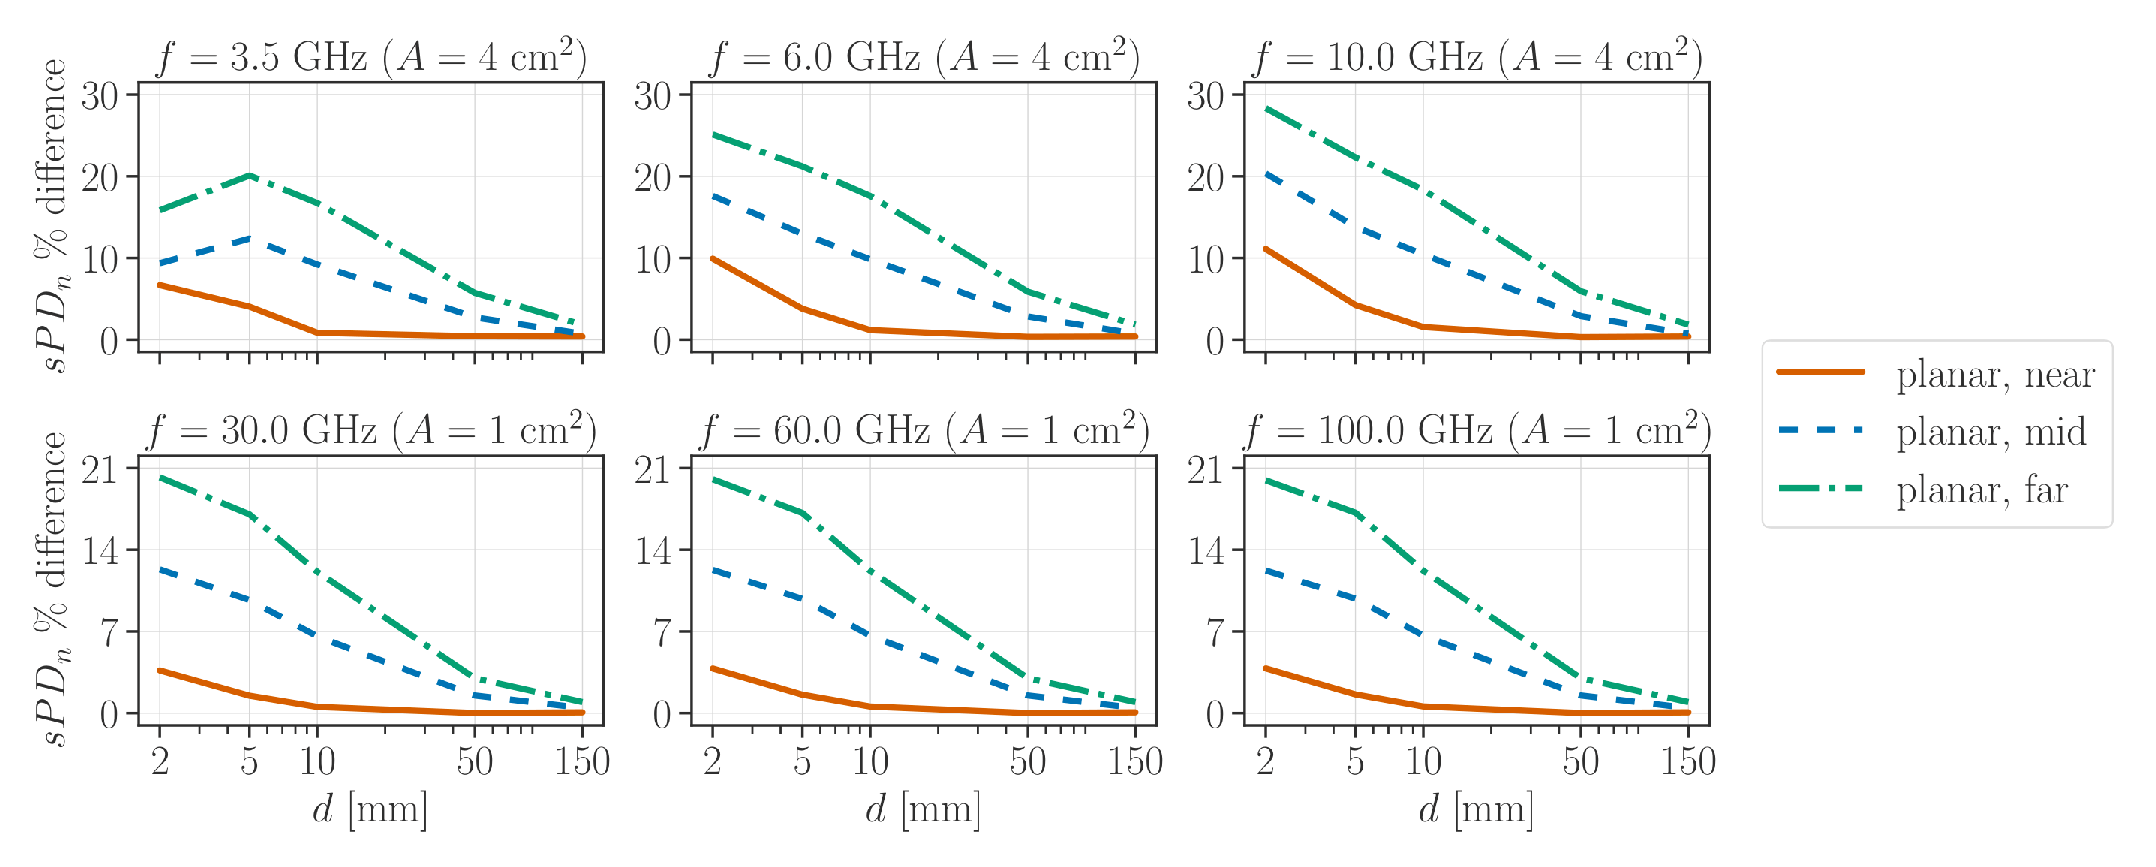
\includegraphics[width=\textwidth]{artwork/IEEE-TEMC-sPDn.pdf}
            \caption{Relative differences averaged over the near-, middle- and far-flat with a spherical surface as functions of the separation distance from the antenna at \SIlist{3.5;6;10;30,60;100}{\GHz}}
        \end{figure}
    \end{onlyenv}
    \begin{onlyenv}<3>
        \begin{figure}
            \centering
            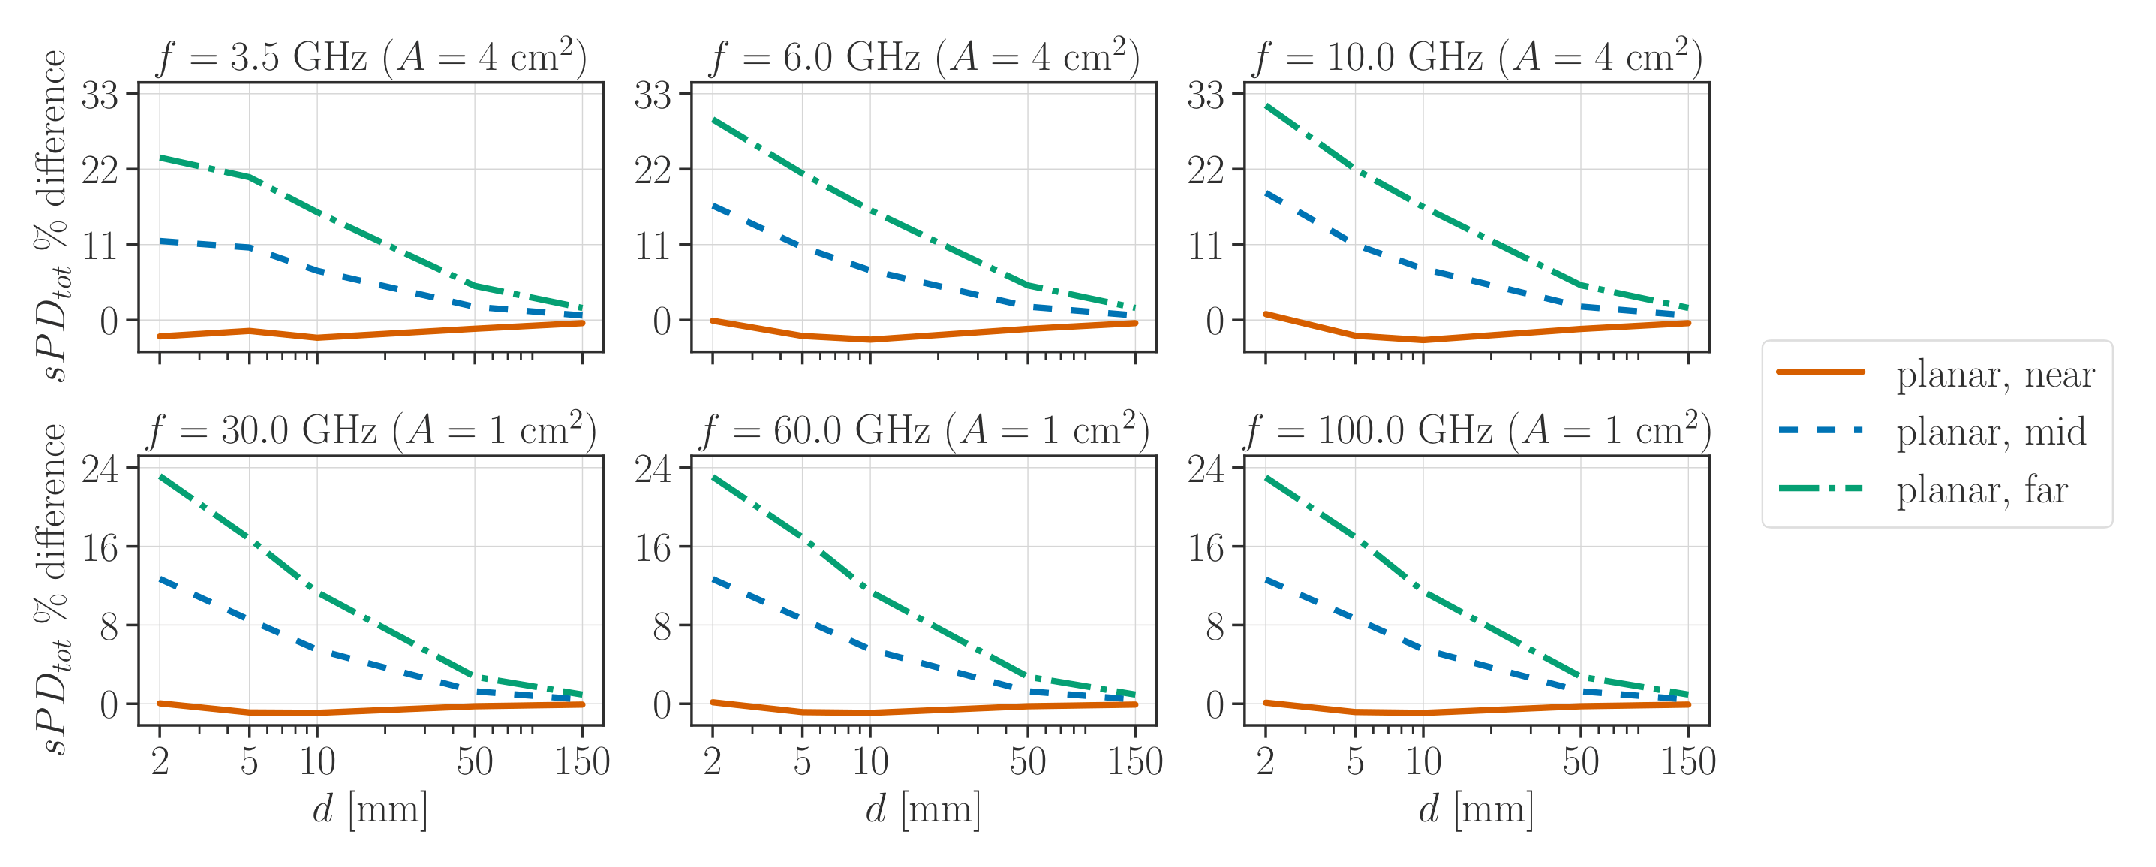
\includegraphics[width=\textwidth]{artwork/IEEE-TEMC-sPDtot.pdf}
            \caption{Relative differences averaged over the near-, middle- and far-flat with a spherical surface as functions of the separation distance from the antenna at \SIlist{3.5;6;10;30,60;100}{\GHz}}
        \end{figure}
    \end{onlyenv}
    \begin{onlyenv}<4>
        Absolute percentage differences between $sPD_\text{n}$ and $sPD_\text{tot}$ on a spherical surface at different separation distances from the antenna at \SIlist{6;30}{\GHz}
        \begin{table}[]
            \centering
            \begin{tabular}{c|c|c|c|c|c|c|}
            \cline{2-7}
             & $d$, \SI{}{\mm} & \num{2} & \num{5} & \num{10} & \num{50} & \num{150} \\ \hline
            \multicolumn{1}{|c|}{\multirow{3}{*}{\SI{6}{\GHz}}} & $sPD_\text{n}$ & 8.30 & 5.54 & 3.03 & 0.22 & 0.03 \\ \cline{2-7} 
            \multicolumn{1}{|c|}{} & $sPD_\text{tot}$ & 12.16 & 6.69 & 3.27 & 0.22 & 0.03 \\ \cline{2-7} 
            \multicolumn{1}{|c|}{} & \% difference${}^*$ & 37.79 & 18.94 & 7.75 & 0.16 & 0.07 \\ \hline
            \multicolumn{1}{|c|}{\multirow{3}{*}{\SI{30}{\GHz}}} & $sPD_\text{n}$ & 27.18 & 12.93 & 4.81 & 0.23 & 0.03 \\ \cline{2-7} 
            \multicolumn{1}{|c|}{} & $sPD_\text{tot}$ & 36.04 & 14.44 & 5.01 & 0.23 & 0.03 \\ \cline{2-7} 
            \multicolumn{1}{|c|}{} & \% difference${}^*$ & 28.04 & 11.07 & 4.02 & 0.06 & 0.02 \\ \hline
            \end{tabular}
        \end{table}
    \end{onlyenv}
\end{frame}

\subsection{Kapetanović and Poljak, \textit{Radiat Prot Dosim}, 2023.}
\begin{frame}{Published paper \#2: Scope}
    Kapetanović, A. and Poljak, D. ``Machine learning-assisted antenna modeling for realistic assessment of incident power density on non-planar surfaces above \SI{6}{\GHz},'' in \textit{Radiat Prot Dosim}, 199(8--9):826--834, 2023, doi: 10.1093/rpd/ncad114
    \begin{itemize}
        \item Utilization of the cylindrical model of a body part
        \item Development of an accurate technique for IPD averaging in cylindrical coordinates
        \item Comparison of the spherical with cylindrical model by using the flat model as a reference
        \item Capturing the effect of the curvature by varying the curvature radius
        \item Upgrading EM simulation of exposure by aiding traditional numerical techniques with machine learning $\rightarrow$ differentiable programming\footcite{Innes2019differentiable}
    \end{itemize}
\end{frame}

\begin{frame}{Published paper \#2: Model and methods}
    \begin{columns}[c]
        \begin{column}{0.4\textwidth}
            \begin{onlyenv}<1>
                \begin{center}
                \begin{figure}
                    \includegraphics[width=\textwidth]{artwork/IEEE-TEMC-dipole.pdf}
                \end{figure}
                \end{center}
            \end{onlyenv}
            \begin{onlyenv}<2>
                \begin{center}
                \begin{figure}
                    \includegraphics[width=\textwidth]{artwork/RPD-network.pdf}
                \end{figure}
                \end{center}
            \end{onlyenv}
            \begin{onlyenv}<3>
                \begin{footnotesize}
                    \begin{equation*}
                        \begin{aligned}
                        E_x = \frac{1}{j4\pi\omega\epsilon_0} \Bigg[{}&  \int_{-\nicefrac{L}{2}}^{\nicefrac{L}{2}} \frac{\partial I(x')}{\partial x'} \frac{\partial g}{\partial x} \; \mathrm{d}x' \\
                        &  -k^2 \int_{-\nicefrac{L}{2}}^{\nicefrac{L}{2}} I(x') g \; \mathrm{d}x' \Bigg]
                        \end{aligned}
                    \end{equation*}
                    \begin{equation*}
                        E_y = \frac{1}{j4\pi\omega\epsilon_0} \int_{-\nicefrac{L}{2}}^{\nicefrac{L}{2}} \frac{\partial I(x')}{\partial x'} \frac{\partial g}{\partial y} \; \mathrm{d}x'
                    \end{equation*}
                    \begin{equation*}
                        E_z = \frac{1}{j4\pi\omega\epsilon_0} \int_{-\nicefrac{L}{2}}^{\nicefrac{L}{2}} \frac{\partial I(x')}{\partial x'} \frac{\partial g}{\partial z} \; \mathrm{d}x'
                    \end{equation*}
                    where
                    \begin{equation*}
                        g = g(x, y, z, x') = \frac{\exp{(-jkR)}}{R},
                    \end{equation*}
                    \begin{equation*}
                        R = \lvert (x'), (x, y, z) \rvert
                    \end{equation*}
                \end{footnotesize}
            \end{onlyenv}
            \begin{onlyenv}<4>
                \begin{center}
                \begin{figure}
                    \includegraphics[width=0.8\textwidth]{artwork/RPD-tissue.pdf}
                \end{figure}
                \end{center}
            \end{onlyenv}
        \end{column} 
        \begin{column}{0.6\textwidth}
            \begin{itemize}
                \item<1> A center-fed half-wavelength dipole, the input power normalized to \SI{10}{\milli\watt}
                \item<2> Current distribution, $I(x')$, governed by the Pocklington integro-differentional equation $\rightarrow$ (a) GB-IBEM, (b) GB-IBEM + neural network for smooth gradients at critical elements
                \item<3> Electric-field components obtained at any point on the surface of the tissue $\rightarrow$ boundary element formalism with automatic differentiation
                \item<4> Reference flat compared to (a) spherical and (b) cylindrical evaluation surfaces
            \end{itemize}
        \end{column}
    \end{columns}  
\end{frame}

\begin{frame}{Published paper \#2: Reported result and takeaways}
    \begin{onlyenv}<1>
        \begin{itemize}
            \item Time-averaged Poynting vector representing the direction and density of EM-power flow into the tissue
            \begin{equation*}
                \mathbf{S} = \frac{1}{2} \Re \left( \mathbf{E} \times \mathbf{H}^{*} \right)
            \end{equation*}
            \item Evaluation surface in cylindrical coordinate system ($r$, $\varphi$, $z$), ISO 80000-2:2019
            \begin{equation*}
                \mathbf{v}(\theta, \varphi) = \left[r \cos(\varphi), r \sin(\varphi), z \right]
            \end{equation*}
            \item Definition: Normal component $\rightarrow$ cylindrical coordinate system
            \begin{equation*}
                sPD_\text{n} = \frac{1}{A} \iint \mathbf{S}(\mathbf{v}) \cdot \left( \mathbf{v}_\varphi \times \mathbf{v}_z \right) \; \mathrm{d}\varphi \mathrm{d}z
            \end{equation*}
        \end{itemize}
    \end{onlyenv}
    \begin{onlyenv}<2>
        \begin{figure}
            \centering
            \includegraphics[width=0.85\textwidth]{artwork/RPD-spdn.pdf}
            \caption{Relative difference in $sPD_\text{n}$ as a function of the separation distance between the spherical and flat, and between the cylindrical and flat  evaluation surface for various curvature radii}
        \end{figure}
    \end{onlyenv}
    \begin{onlyenv}<3>
        Relative difference in $sPD_\text{n}$ at \SI{26}{\GHz} as a function of the separation distance parametrized by curvature radius: (a) flat-spherical, (b) flat-cylindrical
        \begin{columns}[c]
            \begin{column}{0.5\textwidth}
                \begin{center}
                    \begin{figure}
                        \includegraphics[width=0.85\textwidth]{artwork/RPD-radius.pdf}
                    \end{figure}
                \end{center}
            \end{column}
            \begin{column}{0.5\textwidth}
                \begin{center}
                    \begin{figure}
                        \includegraphics[width=\textwidth]{artwork/RPD-exponential.pdf}
                \end{figure}
                \end{center}
            \end{column}
        \end{columns}  
    \end{onlyenv}
\end{frame}

\subsection{Kapetanović et al., \textit{IEEE J Electromagn RF Microw Med Biol}, 2023.}
\begin{frame}{Published paper \#3: Scope}
    Kapetanović, A., Sacco, G. et al. ``Area-averaged transmitted and absorbed power density on a realistic ear model,'' in \textit{IEEE J Electromagn RF Microw Med Biol}, 7(1):39--45, 2023, doi: 10.1109/JERM.2022.3225380
    \begin{itemize}
        \item Utilization of the anatomically detailed adult-human ear model\footcite{Sforza2009Age}
        \item Development of an accurate technique for power-density averaging on arbitrary surfaces
        \item Realization of the (first stage) automatic detection of peak spatial-average power density
        \item Validation of the approach by commercial EM-simulation packages
        \item Comparison of two existing definitions of the spatially averaged APD by considering volumetric and surface integral
        \item Comparison of dosimetric quantities extracted on the surface of the ear with the flat surface used as a reference
    \end{itemize}
\end{frame}

\begin{frame}{Published paper \#3: Model and methods}
    \begin{columns}[c]
        \begin{column}{0.4\textwidth}
            \begin{onlyenv}<1>
                \begin{center}
                \begin{figure}
                    \includegraphics[width=\textwidth]{artwork/IEEE-JERM-ear.pdf}
                \end{figure}
                \end{center}
            \end{onlyenv}
            \begin{onlyenv}<2>
                \begin{center}
                \begin{figure}
                    \includegraphics[width=\textwidth]{artwork/IEEE-JERM-polarization.pdf}
                \end{figure}
                \end{center}
            \end{onlyenv}
        \end{column} 
        \begin{column}{0.6\textwidth}
            \begin{itemize}
                \item<1> Homogeneous adult-human ear model
                \begin{itemize}
                    \item complex permittivity of dry skin: \num{17.71} – j \num{16.87} at \SI{26}{\GHz} and \num{7.98} – $j$ \num{10.90} at \SI{60}{\GHz}\footcite{Gabriel1996Compilation}
                    \item Solution domain discretized by using the tetrahedral mesh (mesh cell length $\sim \nicefrac{\lambda}{8}$) $\rightarrow$ $\sim$ 15M mesh cells in total
                    \item finite element method (FEM)
                \end{itemize}
                \item<2> Exposure to the plane wave with two polarization modes
                \begin{itemize}
                    \item polarization 1 $\rightarrow$ TE-like
                    \item polarization 2 $\rightarrow$ TM-like
                \end{itemize}
            \end{itemize}
        \end{column}
    \end{columns}  
\end{frame}

\begin{frame}{Published paper \#3: Reported result and takeaways}
    \begin{onlyenv}<1>
        \begin{center}
            \begin{figure}
                \includegraphics[width=0.75\textwidth]{artwork/IEEE-JERM-detection.pdf}
            \end{figure}
        \end{center}
    \end{onlyenv}
    \begin{onlyenv}<2>
        \begin{figure}
            \centering
            \includegraphics[width=0.65\textwidth]{artwork/IEEE-JERM-pd.pdf}
            \caption{``Hot-spot'' regions; the top and bottom row correspond to TE- and TM-like polarization, respectively; the first and second column pertains to \SIlist{26;60}{\GHz}, respectively}
        \end{figure}
    \end{onlyenv}
    \begin{onlyenv}<3>
        \begin{figure}
            \centering
            \includegraphics[width=0.75\textwidth]{artwork/IEEE-JERM-rpd.pdf}
            \caption{Relative differences between the two definitions of spatially averaged APD computed on the ear and planar homogeneous skin model}
        \end{figure}
    \end{onlyenv}
\end{frame}

\subsection{Cvetković et al., \textit{J Commun Softw Syst}, 2022.}
\begin{frame}{Published paper \#4: Scope}
    Cvetković, M. et al. ``On the applicability of numerical quadrature for double surface integrals at {5G} frequencies,'' in \textit{J Commun Softw Syst}, 18(1):42--53, 2022, doi: 10.24138/jcomss-2021-0183
    \begin{itemize}
        \item Investigation of the applicability of numerical integration to approximate surface integrals at 5G frequencies
        \item Realization of the comprehensive test suite for multiple combinations of the source and observation triangles
        \item Development of the unit-cube test
        \item Inspection of the effect of increasing frequency and discretization scheme on the convergence of numerical solution (herein the method of moments)
    \end{itemize}
\end{frame}

\begin{frame}{Published paper \#3: Model and methods}
        \begin{columns}[c]
        \begin{column}{0.4\textwidth}
            \begin{onlyenv}<1>
                \begin{footnotesize}
                    \begin{equation*}
                    \begin{aligned}
                        \sum_{n=1}^{N}{}& \left( j \omega \mu_i A_{mn,i} ' \frac{j}{\omega \epsilon_i} B_{mn,i} \right) J_n + \\
                        &+ \sum_{n=1}^{N} \left( C_{mn,i} + D_{mn,i} \right) M_n \\
                        &= \begin{Bmatrix} V_m, \; &i = 1 \\ 0, \; &i = 2 \end{Bmatrix}
                    \end{aligned}
                    \end{equation*}
                \end{footnotesize}
            \end{onlyenv}
            \begin{onlyenv}<2>
                \begin{footnotesize}
                    \begin{equation*}
                    \begin{aligned}
                        A_{mn,i} &= \int_S \mathbf{f}_m \left( \mathbf{r} \right) \cdot \\
                        & \cdot \int_{S'} \mathbf{f}_n \left( \mathbf{r}' \right) G_i(\mathbf{r}, \mathbf{r}') \; \mathrm{d}S' \mathrm{d}S \\
                        B_{mn,i} &= \dots \\
                        C_{mn,i} &= \dots \\
                        D_{mn,i} &= \dots
                    \end{aligned}    
                    \end{equation*}
                \end{footnotesize}
            \end{onlyenv}
            \begin{onlyenv}<3>
                \begin{figure}
                \centering
                \includegraphics[width=0.85\textwidth]{artwork/JCOMSS-cube.pdf}
            \end{figure}
            \end{onlyenv}
        \end{column} 
        \begin{column}{0.6\textwidth}
            \begin{itemize}
                \item<1> The numerical solution of the integral equation-based formulation results in the fully populated system matrix $\rightarrow$ size directly related to the frequency
                \item<2> Numerical solution of the integral equation requires solving multiple double surface integrals
                \item<3> Solution depends on the positional relationship between the surface elements (triangles) $\rightarrow$ unit-cube test
            \end{itemize}
        \end{column}
    \end{columns}  
\end{frame}

\begin{frame}{Published paper \#3: Reported result and takeaways}
    \begin{itemize}
        \item Numerical solution at high-gigahertz frequencies (e.g., at \SI{90}{\GHz}) $\rightarrow$ high quadrature order + ``good enough'' discretization scheme $\rightarrow$ increased demand for matrix storage and fill-time
        \item Optimal quadrature technique $\rightarrow$ low computational demand without sacrificing accuracy of the solution
        \item Reported convergence test $\rightarrow$ automatic selection of the suitable (fine balance between accuracy and efficiency) integration order
    \end{itemize}
\end{frame}

% concluding remarks
\section[Concluding remarks]{Concluding remarks}
\begin{frame}{Concluding remarks}
    \begin{itemize}
        \item more realistic (nonplanar canonical or anatomical) models of human body parts exposed to RF EM fields above 6 GHz, replacing previous flat models
        \item the accurate numerical technique for efficiently evaluating the scalar and vector field surface integrals
        \item the computationally efficient algorithm for automatic detection of ``hot-spots'' regions is developed for proposed models
        \item extensive dosimetric analysis of absorbed and incident EM power density using rigorous mathematical definitions and without simplification of the evaluation surface morphology
    \end{itemize}
\end{frame}

% standout slide for QnA
\begin{frame}{Questions and answers}
    \centering \LARGE \emph{Thank you!}
\end{frame}

% print all references cited in the document
\begin{frame}[allowframebreaks]{References}
  \printbibliography[heading=none]
\end{frame}

\end{document}
